\section{Setting a Baseline}
\subsection{Required submission files}
\begin{enumerate}
	\item \hl{The updated Load-Leveler batch script.}

		\verb!Data/path/to/file!

	\item \hl{The performance plots and description in the report.}

		References to figures here...

\end{enumerate}

\subsection{Questions}
\begin{enumerate}
	\item \hl{Briefly describe the Gaussian Elimination and the provided implementation.}

	Answer...

	\item \hl{How is data distributed among the processes?}

	Answer...

	\item \hl{Explain the changes applied to the provided Load-Leveler batch script.}

	Answer...

	\item \hl{What were the challenges in getting an accurate baseline time for Gaussian Elimination.}

	Answer...

	\item \hl{Describe the compute and MPI times scalability with fixed process counts and varying size of input files for the Sandy Bridge and Haswell nodes. Did you observe any differences?}

	Answer...

	\item \hl{Describe the compute and MPI times scalability with fixed input sets and varying process counts for the Sandy Bridge and Haswell nodes. Did you observe any differences?}

	Answer...

\end{enumerate}

% % Figure example
% \begin{figure}[p] % h=here, t=top, b=bottom, p=(extra)page, !=force
%  	\begin{center}
%  		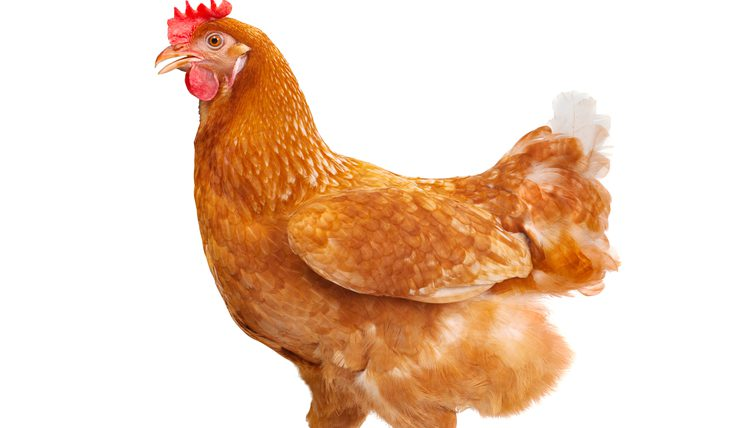
\includegraphics[width=.9\linewidth]{figure.png} % It searches in the Figures/ folder!
%  		\caption{Caption text}
%  		\label{fig:figureLabelName}
%  	\end{center}
% \end{figure}
